\documentclass[english,t]{beamer}
%\documentclass[finnish,english,handout]{beamer}

% Uncomment if want to show notes
% \setbeameroption{show notes}

\mode<presentation>
{
  \usetheme{Warsaw}
  % oder ...
  
  \setbeamercovered{invisible}
  % oder auch nicht
}

% ==============================
%  Added Package
% ==============================
\usepackage[linesnumbered,lined,commentsnumbered]{algorithm2e}
\usepackage{bm}

% =======================================
%   Using symbols for a checklist
% =======================================
\usepackage{pifont}% http://ctan.org/pkg/pifont
\newcommand{\cmark}{\ding{51}}%
\newcommand{\xmark}{\ding{55}}%

% ======================================
%     No Figure in the caption
% ======================================
\setbeamertemplate{caption}{\insertcaption} %---> does not work
%\captionsetup{labelformat=empty,labelsep=none} % ---> it works

% ===================================================
\usepackage{graphicx}
\graphicspath{{./figs/}}
\usepackage[T1]{fontenc}
\usepackage[latin1]{inputenc}
\usepackage{times}
\usepackage{epic,epsfig}
\usepackage{subfigure,float}
\usepackage{amsmath,amsfonts,amssymb}
\usepackage{inputenc}
\usepackage{babel}
\usepackage{afterpage}
\usepackage{eufrak}
\usepackage{amsbsy}
\usepackage{eucal}
\usepackage{rotating}
\usepackage{url}
\urlstyle{same}

\usepackage{natbib}
\bibliographystyle{apalike}

% \definecolor{hutblue}{rgb}{0,0.2549,0.6784}
% \definecolor{midnightblue}{rgb}{0.0977,0.0977,0.4375}
% \definecolor{hutsilver}{rgb}{0.4863,0.4784,0.4784}
% \definecolor{lightgray}{rgb}{0.95,0.95,0.95}
% \definecolor{section}{rgb}{0,0.2549,0.6784}
% \definecolor{list1}{rgb}{0,0.2549,0.6784}
 \definecolor{navyblue}{rgb}{0,0,0.5}
\renewcommand{\emph}[1]{\textcolor{navyblue}{#1}}

% \graphicspath{./pics}

\pdfinfo{            
  /Title      (Bayesian data analysis 2) 
  /Author     (Aki Vehtari) % 
  /Keywords   (Bayesian probability theory, Bayesian inference, Bayesian data analysis)
}


\parindent=0pt
\parskip=8pt
\tolerance=9000
\abovedisplayshortskip=0pt

\setbeamertemplate{navigation symbols}{}
\setbeamertemplate{headline}[default]{}
\setbeamertemplate{headline}[text line]{\insertsection}
\setbeamertemplate{footline}[frame number]


\def\o{{\mathbf o}}
\def\t{{\mathbf \theta}}
\def\w{{\mathbf w}}
\def\x{{\mathbf x}}
\def\y{{\mathbf y}}
\def\z{{\mathbf z}}

\DeclareMathOperator{\E}{E}
\DeclareMathOperator{\Var}{Var}
\DeclareMathOperator{\var}{var}
\DeclareMathOperator{\Sd}{Sd}
\DeclareMathOperator{\sd}{sd}
\DeclareMathOperator{\Gammad}{Gamma}
\DeclareMathOperator{\Invgamma}{Inv-gamma}
\DeclareMathOperator{\Bin}{Bin}
\DeclareMathOperator{\Negbin}{Neg-bin}
\DeclareMathOperator{\Poisson}{Poisson}
\DeclareMathOperator{\Beta}{Beta}
\DeclareMathOperator{\logit}{logit}
\DeclareMathOperator{\N}{N}
\DeclareMathOperator{\U}{U}
\DeclareMathOperator{\BF}{BF}
\DeclareMathOperator{\Invchi2}{Inv-\chi^2}
% \DeclareMathOperator{\Pr}{Pr}
\def\euro{{\footnotesize \EUR\, }}
\DeclareMathOperator{\rep}{\mathrm{rep}}


% ============
% Otsikko sivu
% ============

\title[]{Teori \& Soal KSNP 2020}
\subtitle{}

\author{Hendra Bunyamin}

\institute[  Maranatha]
{
  Teknik Informatika \\
  Fakultas Teknologi Informasi \\
  Universitas Kristen Maranatha
}


\date[NUNI IT Online] % (optional, should be abbreviation of conference name)
{\newline \newline 13 Mei 2022 \\ \bigskip  \bigskip  \bigskip 
\includegraphics[scale=.3]{images/faculty-it-logo}}



%\pgfdeclareimage[height=1.5cm]{university-logo}{images/logo-mcu}
%\logo{\pgfuseimage{university-logo}}
\AtBeginSection[]
{
  \begin{frame}<beamer>{Outline}
    \tableofcontents[currentsection,currentsection]
  \end{frame}
}


\begin{document} 

\begin{frame}
  \titlepage
\end{frame}

%\begin{frame}{Outline}
%  \tableofcontents
%  % You might wish to add the option [pausesections]
%\end{frame}


 \begin{frame}

   \frametitle{Outline dari Sesi ke-3}
  \begin{itemize}
\item Soal 1: Aritmetika Modular 
\item Soal 2: Himpunan
\item Soal 3: Logika
\item Soal 4: Masih Logika
\item Soal 5: Logika Terus?
\bigskip
\item Soal 6: Keliling Bidang Datar
\item Soal 7: Jarak Terpendek
\item Soal 8: Kombinasi Berulang
\item Soal 9: Relasi Rekursif
\item Soal 10: Pemrograman Dinamis
\end{itemize}
\end{frame}

%%%%

%\begin{frame}{Hello World!}
%\begin{algorithm}[H]
%	\SetKwData{Left}{left}
%	\SetKwData{This}{this}
%	\SetKwData{Up}{up}
%	\SetKwFunction{Union}{Union}
%	\SetKwFunction{FindCompress}{FindCompress}
%	\SetKwInOut{Input}{Input}
%	\SetKwInOut{Output}{Output}
%
%\Input{Suatu bil$Im$ of size $w\times l$ \\ and $n$}
%\Output{A partition of the bitmap}
%\BlankLine   
%\emph{special treatment of the first line}\;
%\For{$i\leftarrow 2$ \KwTo $l$}{
%	\emph{special treatment of the first element of line $i$}\;
%	\For{$j\leftarrow 2$ \KwTo $w$}{\label{forins}
%	\Left$\leftarrow$ \FindCompress{$Im[i,j-1]$}\;
%	\Up$\leftarrow$ \FindCompress{$Im[i-1,]$}\;
%	\This$\leftarrow$ \FindCompress{$Im[i,j]$}\;            
%	\If(\tcp*[h]{O(\Left,\This)==1}){\Left compatible with \This}{\label{lt}
%		\lIf{\Left $<$ \This}{\Union{\Left,\This}}
%		\lElse{\Union{\This,\Left}}
%	}
%	\If(\tcp*[f]{O(\Up,\This)==1}){\Up compatible with \This}{\label{ut}
%		\lIf{\Up $<$ \This}{\Union{\Up,\This}}
%		\tcp{\This is put under \Up to keep tree as flat as possible}\label{cmt}
%		\lElse{\Union{\This,\Up}}\tcp*[h]{\This linked to \Up}\label{lelse}
%		}
%	}   
%	\lForEach{element $e$ of the line $i$}{\FindCompress{p}}
%	}
%	\caption{disjoint decomposition}\label{algo_disjdecomp} 
%\end{algorithm}
%\end{frame}

\begin{frame}
  \frametitle{Soal 1: Aritmatika Modular} 
Diberikan sebuah barisan, $1, 4, 5, 16, 17, 20, 21, \ldots$, yang terurut menaik dan terbentuk dari bilangan $4$ pangkat atau penjumlahan dari bilangan $4$ pangkat yang berbeda (contoh: $4^0, 4^1, 4^1 + 4^0, 4^2, 4^2 + 4^0, \ldots$).

\textbf{Tentukan bilangan ke-$\bm{2020}$ yang dimodulo dengan $\bm{31}$}.
%   \begin{center}
%   \only<2>{\includegraphics[width=9cm]{dbinom1.pdf}}
%   \only<3>{\includegraphics[width=9cm]{dbinom10.pdf}}
%   \only<4>{\includegraphics[width=9cm]{dbinom10b.pdf}}
% \end{center}
\end{frame}


\begin{frame}{Soal 2: Diagram Venn}   
Di sebuah sekolah terdapat 4 klub. Berikut penjelasan anggota tiap klub.
\begin{itemize}
	\item Setiap siswa tergabung ke setidaknya satu klub.
	\item Setiap anggota klub $B$ adalah anggota klub $A$.
	\item Sebagian anggota klub $C$ adalah anggota klub $B$.
	\item Semua anggota klub $C$ yang merupakan anggota klub $A$ juga merupakan anggota klub $B$.
	\item Tidak ada anggota klub $D$ yang merupakan anggota klub $A$.
	\item Sebagian anggota klub $D$ adalah anggota klub $C$.
	\item Jumlah seluruh siswa adalah $140$.
	\item Jumlah anggota klub $A$ dan klub $C$ adalah $125$.
	\item Jumlah anggota klub $B$ adalah $40$.
	\item Jumlah anggota klub $D$ adalah $35$.
\end{itemize}
\onslide<2-> \textbf{Berapa jumlah siswa yang merupakan anggota di 1 klub saja?}
\end{frame}

\begin{frame}{Soal 3: Logika}
Ada 6 orang yaitu Albert, Budi, Caca, Danis, Eka, dan Farah, yang masing-masing mengeluarkan sebuah pernyataan yang hanya bisa bernilai benar atau salah saja.

\bigskip
\begin{tabular}{ll}
Albert (A) &: Pernyataanku bernilai benar \\
Budi (B)   &: Antara pernyataan Caca atau Albert \\
Caca (C)   &: Pernyataanku bernilai benar \\
Danis (D)  &: Pernyataan Budi bernilai benar \\
Eka (E)    &: Pernyataan Caca bernilai benar \\
Farah (F)  &: Pernyataanku bernilai benar
\end{tabular} 

\bigskip
Jika \textit{hanya ada tepat 1 pernyataan yang benar dari keenam pernyataan di atas}, pernyataan siapakah yang benar?
\end{frame}



\begin{frame}{Soal 4: Analisis Kemungkinan dengan Logika}
Empat orang sekawan yaitu Kwak, Kwik, Kwek, dan Kwok akan berlibur ke kota Bandung. Akan tetapi karena satu dan lain hal, beberapa (bisa saja tidak ada) dari mereka gagal untuk berlibur ke Kota Bandung. Mereka akhirnya menetapkan aturan berikut untuk menentukan siapa yang akan berlibur ke Kota Bandung

\begin{itemize}
	\item Jika Kwak pergi ke Bandung maka Kwik juga akan ikut ke Bandung.
	\item Hanya tepat salah satu dari Kwik atau Kwek yang akan pergi ke Bandung.
	\item Jika Kwek pergi ke Bandung maka Kwak dan Kwok keduanya harus pergi ke Bandung.
	\item Jika Kwok tidak pergi ke Bandung, maka Kwik juga tidak akan pergi ke Bandung.
\end{itemize}

Berapa banyak kemungkinan orang-orang yang akan pergi ke Bandung?
\end{frame}

\begin{frame}{Soal 5: Operasi Logika}
Perhatikan operasi logika berikut!
\begin{align*}
P &= (A \text{ AND }(\text{NOT }B)) \text{ OR }((C \text{ OR }(\text{ NOT }D)) \text{ AND } (\text{ NOT }E)) \\
Q &= ((\text{NOT }A) \text{ OR }(\text{NOT }B)) \text{ AND }(((\text{NOT }C) \text{ AND }D) \text{ OR }(\text{NOT } E))  \\
R &= P \text{ AND }Q.
\end{align*}
Jika $A$ = True, $B$ = True, $C$ = True, $D$ = True, dan $E$ = False. Tentukan nilai $P$, $Q$, dan $R$ berturut-turut?
\end{frame}


\begin{frame}{Soal 6: Keliling Terkecil}
Pak Dengklek memiliki 8 titik yang terletak pada koordinat:
\begin{equation*}
(2,5), (3,8), (3,4), (4,8), (4,0), (3,3), (0,4), (0,0)
\end{equation*}
Beliau ingin menutupi kedelapan titik tersebut dengan sebuah poligon sedemikian sehingga setiap titik milik Pak Dengklek berada di dalam (atau di tepi) poligon tersebut. 

\bigskip
Berapa \textit{keliling poligon terkecil} yang memenuhi keinginan Pak Dengklek?
\end{frame}


\begin{frame}{Soal 7: Algoritma Dijkstra (1/2)} 
Kerajaan Zidan sedang berperang melawan Kerajaan Ahmad. Salah satu mata-mata Kerajaan Zidan berhasil mendapatkan peta logistik Kerajaan Ahmad, yaitu sebagai berikut:
\begin{figure}[!ht]
	\centering
	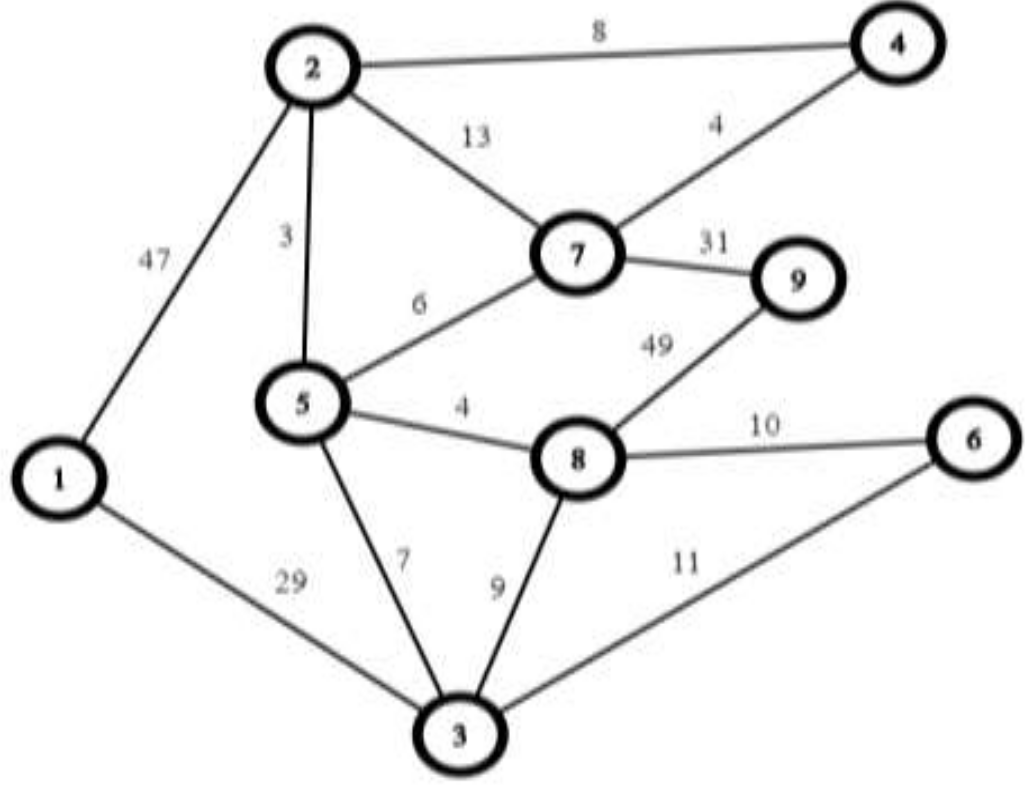
\includegraphics[scale=.225]{images/soal-7-peta}
\end{figure}
\end{frame}

\begin{frame}{Soal 7: Algoritma Dijkstra (2/2)} 
Sumber logistik Kerajaan Ahmad berada di node bernomor 1 dan Kerajaan Ahmad berada di node bernomor 9. Kerajaan Zidan ingin memutus jalur logistik Kerajaan Ahmad agar memenangkan perang. Dengan kata lain, Kerajaan Zidan ingin menghancurkan beberapa jalan sedemikian sehingga tidak ada jalan yang bisa digunakan untuk mencapai node 9 dari node 1, dan sebaliknya. Bilangan yang tertera pada jalan merupakan biaya yang dibutuhkan Kerajaan Zidan untuk menghancurkan jalan tersebut. 

\bigskip
\textit{Berapa total biaya minimum yang dibutuhkan Kerajaan Zidan?}
\end{frame}


\begin{frame}{Soal 8: Permutasi}
Terdapat 4 ekor bebek berwarna merah, 3 ekor bebek berwarna biru, dan 2 ekor bebek berwarna hijau. Kesembilan bebek tersebut diminta untuk berbaris oleh Pak Dengklek dengan ketentuan:

\begin{itemize}
	\item Setiap bebek yang berwarna sama tidak bisa dibedakan.
	\item Untuk setiap pasang bebek yang berwarna sama, tidak boleh ada bebek lain yang warnanya berbeda yang berada di antara sepasang bebek tersebut.
\end{itemize}

\bigskip
\textit{Ada berapa macam posisikah yang mungkin dalam barisan bebek tersebut?}
\end{frame}


\begin{frame}{Soal 9: Teknik Analisis Rekursif}
Pak Dengklek memiliki sebuah fungsi $f$ yang dapat dinyatakan sebagai berikut:
\begin{equation*}
f(n) =
\left\{ \begin{array}{rcl}
1                       & \mbox{for} & n \leq 1 \\ 
f(\frac{n}{2}) * 2 + n, & \mbox{for} & n > 1
\end{array}\right.
\end{equation*}
Berapakah nilai $f(1048576)$?
\end{frame}


\begin{frame}{Soal 10: Pemrograman Dinamis}
Pak Dengklek memiliki sebuah sekuens $S = \{2, 14, 7, 20, 5, 3, 8, 11, 18, 4, 10, 12, 1, 6, 9, 19, 15, 16, 13, 17\}$. \\
Subsekuens dari sebuah sekuens $S$ bisa didapatkan dengan menghilangkan beberapa elemen dari $S$ namun dengan tetap mempertahankan urutannya. Sebagai Contoh: $\{2, 7, 13, 17\}$ adalah subsekuens dari $S$, sedangkan $\{14, 2, 20\}$ bukanlah subsekuens dari $S$ karena urutannya berubah (2 muncul lebih dahulu dari 14 di $S$).

\bigskip
Pak Dengklek ingin mencari sebuah subsekuens menaik dari $S$. Sebuah subsekuens dikatakan menaik jika dan hanya jika elemen-elemen yang ada di dalam subsekuens tersebut tersusun secara menaik. Sebagai Contoh: $\{2, 7, 20\}$. 

\bigskip
Berapa banyaknya elemen dari subsekuens menaik terpanjang yang bisa dibentuk dari sekuens $S$?
\end{frame}


%%%% predictive distribution


 % \begin{frame}
 %   \frametitle{Some other one parameter models}

 %   \begin{itemize}
 %   \item Poisson
 %   \item Exponential
 %   \item Cauchy
 %   \end{itemize}
   
 % \end{frame}

%\section<presentation>*{\appendixname}
%\subsection<presentation>*{For Further Reading}
%
%\begin{frame}[allowframebreaks]
%  \frametitle<presentation>{Daftar Pustaka}
%    {\footnotesize
%%    \bibliographystyle{apalike}
%    \bibliography{references}
%    }    
%\end{frame}

\end{document}

%%% Local Variables: 
%%% TeX-PDF-mode: t
%%% TeX-master: t
%%% End: 
